\section{Shock wave simulation}
We studied the evolution of trans-relativistic shocks and spectum of accelerated particles. We chose relastivistic shocks with low lorenz-factor because the maximum energy of produced cosmic rays increases with shock wave lorenz-factor, but the efficiency of acceleration decreases, because it is more difficult for particle to cross fast moving front many times \cite{Ellison2013}. So we assume that intermediate case of trans-relativistic shocks provides the most effective acceleration.

We developed the implicit particle-in-cell (PIC) code, presented in our previous paper \cite{Romansky2016}, based on the scheme suggested by Lapenta et al.~\cite{Lapenta2006} and improved for the relativistic case by Noguchi et al.\cite{Noguchi2007}.
Our code is fully three dimensional and parallelized with MPI technology, which is adapted for distributed computing and can be executed on a wide class of computers.

In simulation setup the homogeneous plasma flows in through the right boundary
and collides with the reflecting superconducting wall on the left boundary, causing the shock wave
  

\begin{figure}[h!]
	\centering
	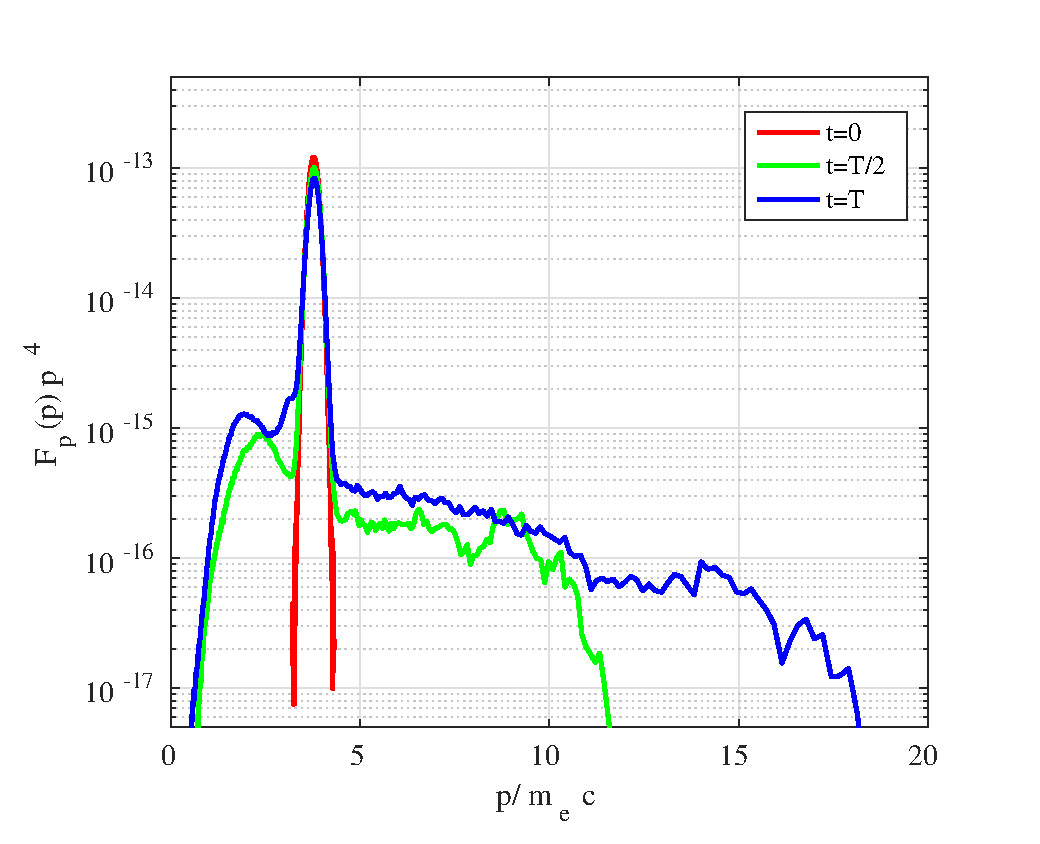
\includegraphics[width=0.86\textwidth]{fig/protons.eps} 
	\caption{Distribution of protons.}
	\label{protons}
\end{figure}
\begin{figure}[h!]
	\centering
	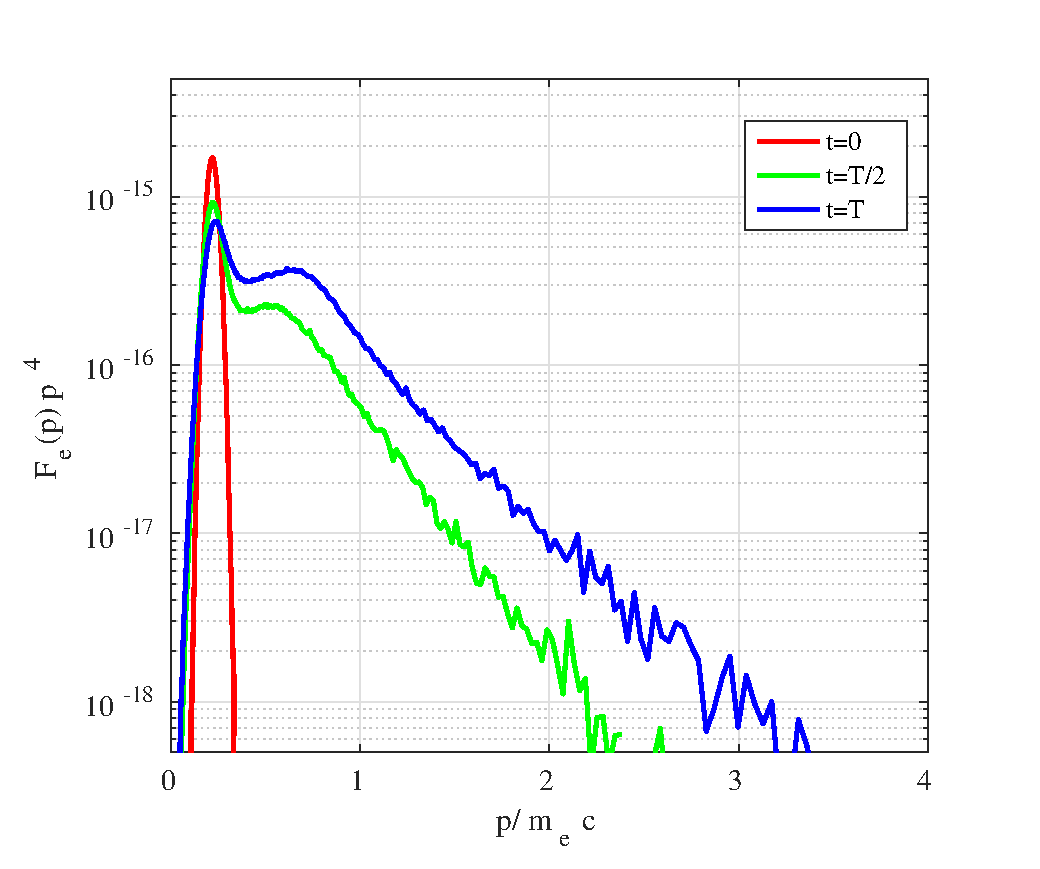
\includegraphics[width=0.86\textwidth]{fig/electrons.eps} 
	\caption{Distribution of electrons.}
	\label{electrons}
\end{figure}

Simulations are one-dimensional and have following parameters: initial flow lorenz-factor $\gamma = 1.5$, number densities $n_e = 10^{-4} \rm{cm}^{-3}$, $n_p = 10^{-4} \rm{cm}^{-3}$ , temperature $5\cdot10^8 \rm{K}$, magnetic field $B = 10^{-4} \rm{G}$, the full size of the box $L = 2\cdot10^{12} \rm{cm}$, the number of cells $N=2\cdot10^4$. Electron mass is reduced to $m_e = \frac{m_p}{20}$. The full time of simulation is $T = 5000 {\omega_p}^{-1}$. $\theta$ is angle between flow velocity and magnetic field. We present results of particle spectrum in several simulations with different $\theta$. 

One can see from Figures \ref{protons} and \ref{electrons} that spectrum of accelerated particles strongly depends on angle theta. If $\theta$ is less then critical value, defined by equation $c\cdot cos(\theta_{crit})=v_{shock}$, where all values are measured in upstream rest frame, particles can escape from the front and cross it several times to gain more energy. It is difficult to evaluate critical angle apriori, because we don't know compression relation of shock wave which will be created in simulation, but estimation for case of strong wave (comression relation $\sigma=4^{\circ}$) gets $\theta_{crit}=45$ in downstream frame. And it is consistent with results of our simulations.

